% ============================================================================
%  COMPILE WITH XeLaTeX  (twice, so the point total resolves)
%  Overleaf: Menu -> Compiler -> XeLaTeX
%  Requires: bnhandout.sty and fonts/Kalpurush.ttf in the project
% ============================================================================
\documentclass[11pt]{article}
\usepackage{bnhandout}          % add [nosol] for a student edition

\hauthor[https://sites.google.com/view/jugantordey/home]{Jugantor Dey}
\hseries{\textit{Mathematics for the Physics Olympiad}}

\begin{document}

\handouttitle{Chapter 10 : Function II}

\noindent
শুরু করার আগে ৪ নম্বর অধ্যায় থেকে domain, range, এক-এক ও সার্বিক ফাংশন এবং
বিপরীত ফাংশনের সংজ্ঞাগুলো, আর ৮ নম্বর অধ্যায় থেকে ভগ্নাংশ সূচক, লগারিদমের
নিয়ম ও $e$ সংখ্যাটি একবার দেখে নাও। ওখানে $\log$ ছিল একটা হিসাবের যন্ত্র; এখানে
সেটি একটি ফাংশন হয়ে উঠবে, আর তার সবটুকু ভর বইবে ৪ নম্বর অধ্যায়ের বিপরীত
ফাংশনের যন্ত্রপাতি।

এই অধ্যায়ের বিষয় দুটি ফাংশন: $e^{x}$ এবং $\ln x$। পদার্থবিজ্ঞানে যত ফাংশন
আসে তার মধ্যে এই দুটি সম্ভবত সবচেয়ে বেশি আসে, কারণ প্রকৃতিতে যেখানেই কোনো রাশির
পরিবর্তনের হার তার নিজের পরিমাণের সমানুপাতিক, সেখানেই এরা হাজির হয়:
তেজস্ক্রিয় ক্ষয়, ধারকের চার্জ হারানো, বায়ুমণ্ডলের চাপ, জনসংখ্যা। শেষ দুটি
অনুচ্ছেদে আমরা একটু সরে গিয়ে দেখব কীভাবে যেকোনো একটি চেনা লেখচিত্র থেকে গোটা
পরিবার তৈরি করা যায়, এবং প্রতিসাম্য কীভাবে কাজ অর্ধেক করে দেয়। এই অধ্যায়ে
মোট \totalpoints\ পয়েন্ট আছে।

\section{সূচকীয় ফাংশন}

দুটি রাশি দেখতে প্রায় একরকম, অথচ চরিত্রে সম্পূর্ণ আলাদা: $x^{a}$ এবং $a^{x}$।
প্রথমটিতে চলকটি নিচে, ঘাত ধ্রুবক; একে বলে power function। দ্বিতীয়টিতে চলকটি
উপরে, ভিত্তি ধ্রুবক; একে বলে exponential function। এই অনুচ্ছেদ পুরোটাই
দ্বিতীয়টিকে নিয়ে।

\begin{idea}[সূচকীয় ফাংশন]
$a > 0$ এবং $a \neq 1$ হলে
\[
  f \colon \mathbb{R} \to (0, \infty), \qquad f(x) = a^{x}
\]
ফাংশনটিকে বলে $a$ ভিত্তির exponential function। এর domain সমগ্র $\mathbb{R}$,
এবং range হলো $(0,\infty)$, অর্থাৎ মান কখনো ঋণাত্মক বা শূন্য হয় না।
\end{idea}

একটা সততার কথা এখানে বলে রাখা দরকার। ৮ নম্বর অধ্যায়ে আমরা $a^{p/q}$ সংজ্ঞায়িত
করেছি মূলদ ঘাতের জন্য, $a^{p/q} = \sqrt[q]{a^{p}}$ ধরে। কিন্তু $a^{\sqrt{2}}$
মানে কী? ইন্টুইশনটা হলো, $\sqrt{2}$-এর কাছাকাছি মূলদ সংখ্যাগুলোর
($1.4$, $1.41$, $1.414$, \dots) ঘাতগুলো একটি নির্দিষ্ট সংখ্যার দিকে এগোয়, আর
সেটিকেই $a^{\sqrt{2}}$ বলা হয়। এই ``এগোয়'' কথাটির সঠিক অর্থ limit, যা ১৪ নম্বর
অধ্যায়ের বিষয়। আপাতত আমরা \emph{ধরে নিচ্ছি} যে এভাবে সব বাস্তব $x$-এর জন্য
$a^{x}$ সংজ্ঞায়িত করা যায় এবং ৮ নম্বর অধ্যায়ের সূচকের সব নিয়ম তখনো খাটে।

\begin{idea}[সূচকীয় ফাংশনের চরিত্র]
$f(x) = a^{x}$-এর জন্য
\[
  f(x+y) = f(x)\,f(y), \qquad f(0) = 1, \qquad f(-x) = \frac{1}{f(x)} .
\]
প্রথম সমীকরণটিই এই ফাংশনের আসল পরিচয়: \emph{যোগফলকে সে গুণফলে বদলে দেয়}।
এর সরাসরি ফল হলো, যেকোনো নির্দিষ্ট $h$-এর জন্য
\[
  \frac{f(x+h)}{f(x)} = a^{h},
\]
যা $x$-এর উপর একেবারেই নির্ভর করে না। অর্থাৎ সমান ব্যবধিতে রাশিটি সমান
\emph{গুণিতকে} বাড়ে বা কমে, সমান পরিমাণে নয়।
\end{idea}

এই শেষ বাক্যটিই সূচকীয় বৃদ্ধি আর সরলরৈখিক বৃদ্ধির পার্থক্য। সরলরেখায় প্রতি ধাপে
একই পরিমাণ \emph{যোগ} হয়; সূচকীয় ফাংশনে প্রতি ধাপে একই সংখ্যা দিয়ে \emph{গুণ}
হয়।

কয়েকটি ধর্ম সহজেই দেখা যায়। প্রথমত $a^{x} > 0$ সব $x$-এর জন্য, কারণ
$a^{x} = \left( a^{x/2} \right)^{2}$ একটি বর্গ, আর সেটি শূন্যও হতে পারে না
(শূন্য হলে $a^{x/2} = 0$ হতো, অথচ $a^{x/2} \cdot a^{-x/2} = 1$)। দ্বিতীয়ত
$a > 1$ হলে $h > 0$-এর জন্য $a^{h} > 1$, সুতরাং
$a^{x+h} = a^{x} \cdot a^{h} > a^{x}$; অর্থাৎ ফাংশনটি কড়াভাবে বর্ধমান। একইভাবে
$0 < a < 1$ হলে এটি কড়াভাবে হ্রাসমান। কড়া একঘেয়েমি (strictly monotone) মানেই
এক-এক, তাই ৪ নম্বর অধ্যায়ের ভাষায় $a^{x}$ একটি injective ফাংশন। এটিই
আমাদের ``দুই পাশের ঘাত সমান করে দাও'' নিয়মটি ব্যবহারের অনুমতি দেয়:
$a^{u} = a^{v}$ হলে অবশ্যই $u = v$।

\begin{center}
\begin{tikzpicture}[x=1.05cm,y=0.72cm,>=stealth]
  \draw[thick,->] (-2.4,0) -- (2.7,0) node[below] {$x$};
  \draw[thick,->] (0,-0.5) -- (0,5.5) node[right] {$y$};
  \foreach \x in {-2,-1,1,2} \draw (\x,0.1) -- (\x,-0.1) node[below] {$\x$};
  \foreach \y in {1,2,3,4,5} \draw (0.08,\y) -- (-0.08,\y) node[left] {$\y$};
  \begin{scope}
    \clip (-2.4,-0.4) rectangle (2.4,5.2);
    \draw[thick,domain=-2.4:2.4,smooth,variable=\x] plot ({\x},{exp(0.6931*\x)});
    \draw[thick,domain=-2.4:1.7,smooth,variable=\x] plot ({\x},{exp(\x)});
    \draw[thick,domain=-2.4:2.4,smooth,variable=\x] plot ({\x},{exp(-0.6931*\x)});
  \end{scope}
  \draw[dashed] (-2.4,0) -- (2.4,0);
  \draw[fill] (0,1) circle (1.6pt);
  \node[right] at (1.72,4.5) {$y=e^{x}$};
  \node[right] at (2.05,3.3) {$y=2^{x}$};
  \node[left] at (-1.95,3.3) {$y=\left(\tfrac{1}{2}\right)^{x}$};
\end{tikzpicture}
\end{center}

ছবিতে তিনটি লেখচিত্রই $(0,1)$ বিন্দু দিয়ে যাচ্ছে, কারণ $a^{0} = 1$ সব $a$-এর
জন্য। $a > 1$ হলে লেখচিত্র ডানদিকে উঠে যায় আর বামদিকে $x$-অক্ষের গা ঘেঁষে
নামতে থাকে, কখনো ছোঁয় না; $x$-অক্ষটি তাই একটি horizontal asymptote। ``ছোঁয় না
অথচ যত কাছে ইচ্ছা যায়'' কথাটির নির্ভুল অর্থও limit, তাই এখানে asymptote শব্দটি
আমরা অনানুষ্ঠানিকভাবেই ব্যবহার করছি; ১৪ নম্বর অধ্যায়ে এটি সংজ্ঞায়িত হবে।

\begin{example}
$4^{x+1} = 8^{x-1}$ সমীকরণটি সমাধান করো।
\end{example}

\begin{solbox}
দুই পাশকে একই ভিত্তিতে আনি। $4 = 2^{2}$ এবং $8 = 2^{3}$, তাই
\[
  2^{2(x+1)} = 2^{3(x-1)} .
\]
$2^{x}$ ফাংশনটি এক-এক, তাই ঘাত দুটি সমান হতেই হবে: $2x + 2 = 3x - 3$, অর্থাৎ
$x = 5$। যাচাই: বাম পাশ $4^{6} = 4096$, ডান পাশ $8^{4} = 4096$।

খেয়াল করো, ``ঘাত সমান করে দাও'' ধাপটি কোনো সূত্র নয়, এটি এক-এক হওয়ার ফল।
$a = 1$ হলে $1^{u} = 1^{v}$ সব $u, v$-এর জন্যই সত্য হতো, আর তখন এই ধাপটি ভুল
হতো; এই কারণেই সংজ্ঞায় $a \neq 1$ শর্তটি রাখা হয়েছে।
\end{solbox}

\begin{example}
$f(x) = a^{x}$ ধরনের একটি ফাংশনের জন্য $f(1) = 5$ দেওয়া আছে। কেবল
$f(x+y) = f(x)f(y)$ সম্পর্কটি ব্যবহার করে $f(3)$, $f(0)$ ও $f(-1)$ বের করো।
\end{example}

\begin{solbox}
$f(3) = f(1+1+1) = f(1)f(1)f(1) = 5^{3} = 125$।

$f(0)$-এর জন্য লিখি $f(1) = f(1+0) = f(1) f(0)$; যেহেতু $f(1) = 5 \neq 0$, দুই
পাশকে $5$ দিয়ে ভাগ করে $f(0) = 1$।

$f(-1)$-এর জন্য $1 = f(0) = f(1 + (-1)) = f(1) f(-1) = 5 f(-1)$, সুতরাং
$f(-1) = \tfrac{1}{5}$।

মজার ব্যাপার হলো, $a$ কত তা আমাদের জানতে হয়নি; শুধু ঐ একটি সম্পর্ক আর একটি মান
থেকেই সব বেরিয়ে এসেছে।
\end{solbox}

\begin{remark}
সব ভিত্তির মধ্যে $e$ কেন বিশেষ? ৮ নম্বর অধ্যায়ে $e$-কে সংখ্যাগতভাবে
পরিচয় করানো হয়েছিল। ফাংশন হিসেবে তার বিশেষত্ব একটাই: $y = a^{x}$ লেখচিত্রটি
$(0,1)$ বিন্দুতে যে ঢালে $y$-অক্ষ পার হয়, সেই ঢাল ঠিক $1$ হয় কেবল $a = e$
হলে। $2^{x}$-এর ক্ষেত্রে ঐ ঢাল প্রায় $0.693$, $3^{x}$-এর ক্ষেত্রে প্রায়
$1.099$, আর মাঝামাঝি কোথাও ঢালটি ঠিক $1$ হয়; সেই ভিত্তিটাই $e \approx 2.71828$।
এর ফলে $e^{x}$ হলো একমাত্র সূচকীয় ফাংশন যার পরিবর্তনের হার হুবহু সে নিজেই।
এই বাক্যটির অর্থ ও প্রমাণ দুটোই ১৫ নম্বর অধ্যায়ের, কারণ ``ঢাল'' মাপতে
derivative লাগে; এখানে একে আমরা $e$ বেছে নেওয়ার কারণ হিসেবে ধরে নিচ্ছি।
\end{remark}

\begin{remark}
আরেকটি ব্যাপার এখনই গেঁথে নেওয়া ভালো: সূচকীয় ফাংশন যেকোনো power function-কে
শেষ পর্যন্ত হারিয়ে দেয়। $x = 10$-এ $x^{10} = 10^{10}$ আর $2^{x} = 1024$, অর্থাৎ
power এগিয়ে; কিন্তু $x = 100$-এ $x^{10} = 10^{20}$ আর
$2^{x} \approx 1.3 \times 10^{30}$, অর্থাৎ প্রায় $10^{10}$ গুণ বেশি। যত বড় ঘাতই নাও, একটা
জায়গার পরে সূচকীয় ফাংশনই জেতে। এটি এখানে প্রমাণ করা হচ্ছে না; সংখ্যা দেখে
মেনে নেওয়া হচ্ছে, আর ১৫ নম্বর অধ্যায়ের হাতিয়ার দিয়ে এটি ঠিকভাবে দেখানো
যাবে।
\end{remark}

\prob{2} সমাধান করো।
\begin{enumerate}
  \item $2^{3x-1} = 32$
  \item $9^{x} = 27^{x-1}$
  \item $5^{x^{2}-3x} = \dfrac{1}{25}$
\end{enumerate}

\begin{sol}
\begin{enumerate}
  \item $32 = 2^{5}$, তাই $3x - 1 = 5$, অর্থাৎ $x = 2$।
  \item $3^{2x} = 3^{3(x-1)}$, তাই $2x = 3x - 3$, অর্থাৎ $x = 3$।
  \item $\dfrac{1}{25} = 5^{-2}$, তাই $x^{2} - 3x = -2$, অর্থাৎ
        $x^{2} - 3x + 2 = 0$, অর্থাৎ $(x-1)(x-2) = 0$। সুতরাং $x = 1$ বা
        $x = 2$।
\end{enumerate}
তিনটি ক্ষেত্রেই ঘাত সমান করার অনুমতি এসেছে সূচকীয় ফাংশনের এক-এক হওয়া থেকে।
\end{sol}

\prob{2} $f(x) = a^{x}$ এবং $g(x) = x^{2}$ ধরো।
\begin{enumerate}
  \item দেখাও যে $\dfrac{f(x+h)}{f(x)}$ রাশিটি $x$-এর উপর নির্ভর করে না।
  \item দেখাও যে $\dfrac{g(x+h)}{g(x)}$ রাশিটি $x$-এর উপর নির্ভর করে।
\end{enumerate}
এই পার্থক্যটি এক বাক্যে ব্যাখ্যা করো।

\begin{sol}
\begin{enumerate}
  \item $\dfrac{a^{x+h}}{a^{x}} = a^{x+h-x} = a^{h}$, যেখানে $x$ নেই।
  \item $\dfrac{(x+h)^{2}}{x^{2}} = \left( 1 + \dfrac{h}{x} \right)^{2}$, যেখানে
        $x$ স্পষ্টভাবেই আছে। যেমন $h = 1$ নিলে $x = 1$-এ মান $4$, কিন্তু
        $x = 10$-এ মান $1.21$।
\end{enumerate}
পার্থক্যটি হলো: সূচকীয় ফাংশনে সমান ব্যবধিতে সমান গুণিতক আসে, যেখানে থেকেই শুরু
করা হোক না কেন; power function-এ তা হয় না, সেখানে শুরুর জায়গাটা গুরুত্বপূর্ণ।
\end{sol}

\prob{3} কোনটি বড়, $2^{100}$ না $100^{20}$? উত্তরটি ক্যালকুলেটর ছাড়া যুক্তি দিয়ে
দাও। এরপর ৯ নম্বর অধ্যায়ের আরোহ ব্যবহার করে প্রমাণ করো যে সব পূর্ণসংখ্যা
$n \geq 5$-এর জন্য $2^{n} > n^{2}$।

\begin{sol}
প্রথম অংশ: $2^{100} = \left( 2^{5} \right)^{20} = 32^{20}$, আর $32 < 100$, তাই
$32^{20} < 100^{20}$। সুতরাং $100^{20}$ বড়।

দ্বিতীয় অংশ, আরোহ দিয়ে।

\textbf{ভিত্তি ধাপ।} $n = 5$-এ $2^{5} = 32 > 25 = 5^{2}$।

\textbf{আরোহ ধাপ।} ধরি $k \geq 5$ এবং $2^{k} > k^{2}$। তাহলে
\[
  2^{k+1} = 2 \cdot 2^{k} > 2k^{2} .
\]
এখন দেখাই যে $2k^{2} \geq (k+1)^{2}$। এটি সমান কথা $k^{2} - 2k - 1 \geq 0$,
অর্থাৎ $(k-1)^{2} \geq 2$; আর $k \geq 5$ হলে $(k-1)^{2} \geq 16$, সুতরাং শর্তটি
মানা হয়। অতএব $2^{k+1} > (k+1)^{2}$, এবং আরোহ অনুযায়ী ফলটি সব $n \geq 5$-এর
জন্য সত্য।

লক্ষ করো, দুটি অংশ একে অপরের বিরোধী নয়। $n = 100$-এ $2^{100} > 100^{2}$ সত্যিই
সত্য; কিন্তু $100^{20}$ অনেক বড় একটি রাশি, আর সূচকীয় ফাংশনকে তাকে ছাড়িয়ে যেতে
আরও বড় $n$ লাগে।
\end{sol}

\section{লগারিদমীয় ফাংশন}

\begin{idea}[লগারিদম একটি বিপরীত ফাংশন]
$a > 0$, $a \neq 1$ হলে $f(x) = a^{x}$ ফাংশনটি $\mathbb{R}$ থেকে $(0,\infty)$-এ
একটি bijection। তাই ৪ নম্বর অধ্যায় অনুযায়ী তার একটি বিপরীত ফাংশন আছে:
\[
  \log_{a} \colon (0,\infty) \to \mathbb{R}, \qquad
  \log_{a} x = y \iff a^{y} = x .
\]
$a = e$ হলে একে লেখা হয় $\ln x$ এবং বলা হয় natural logarithm। বিপরীত ফাংশনের
সংজ্ঞা থেকেই সরাসরি পাই
\[
  \ln \left( e^{x} \right) = x , \qquad e^{\ln x} = x .
\]
প্রথমটি সব বাস্তব $x$-এর জন্য খাটে, দ্বিতীয়টি কেবল $x > 0$-এর জন্য।
\end{idea}

এখানে একটি ধাপ ধার করা হয়েছে, সেটি বলে রাখি। $a^{x}$ যে এক-এক, তা আমরা উপরে
দেখিয়েছি। কিন্তু তার range যে ঠিক পুরো $(0,\infty)$, অর্থাৎ প্রতিটি ধনাত্মক
সংখ্যাই কোনো না কোনো $a^{y}$ আকারে পাওয়া যায়, সেটি প্রমাণ করতে ধারাবাহিকতার
একটি উপপাদ্য লাগে যা ১৪ নম্বর অধ্যায়ে আসবে। আপাতত এটি ধরে নেওয়া হচ্ছে;
লেখচিত্র দেখলে ব্যাপারটা বিশ্বাসযোগ্য মনে হয়, কারণ বাঁ দিকে সে $0$-এর দিকে নামে
আর ডান দিকে যত ইচ্ছা উপরে ওঠে, মাঝখানে কোনো লাফ না দিয়ে।

\begin{center}
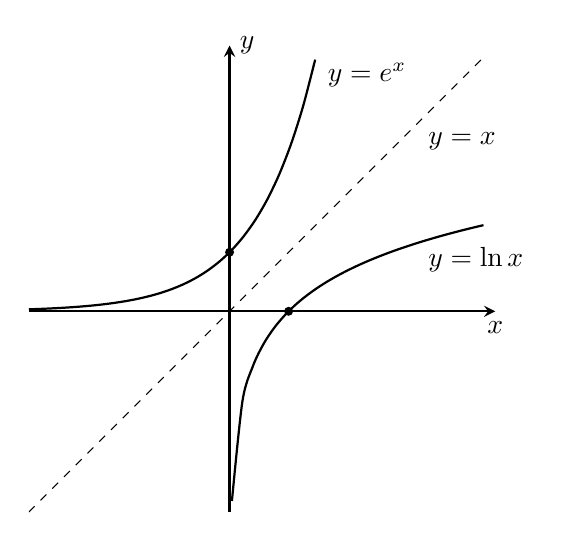
\begin{tikzpicture}[x=0.75cm,y=0.75cm,>=stealth]
  \draw[thick,->] (-3.4,0) -- (4.5,0) node[below] {$x$};
  \draw[thick,->] (0,-3.4) -- (0,4.5) node[right] {$y$};
  \begin{scope}
    \clip (-3.4,-3.4) rectangle (4.3,4.3);
    \draw[thick,domain=-3.4:1.45,smooth,variable=\x] plot ({\x},{exp(\x)});
    \draw[thick,domain=0.04:4.3,smooth,variable=\x] plot ({\x},{ln(\x)});
    \draw[dashed] (-3.4,-3.4) -- (4.3,4.3);
  \end{scope}
  \node[right] at (1.5,4.0) {$y=e^{x}$};
  \node[below right] at (3.2,1.25) {$y=\ln x$};
  \node[below right] at (3.2,3.2) {$y=x$};
  \draw[fill] (0,1) circle (1.4pt);
  \draw[fill] (1,0) circle (1.4pt);
\end{tikzpicture}
\end{center}

$f^{-1}$-এর লেখচিত্র হলো $f$-এর লেখচিত্রকে
$y = x$ রেখায় প্রতিফলিত করলে যা পাওয়া যায়। ছবিটি ঠিক তাই দেখাচ্ছে। এর ফলে
$e^{x}$-এর প্রতিটি ধর্ম আয়নায় উল্টে $\ln x$-এর ধর্ম হয়ে যায়: domain $(0,\infty)$,
range $\mathbb{R}$, লেখচিত্র $(1,0)$ বিন্দু দিয়ে যায়, ফাংশনটি বর্ধমান, এবং
$y$-অক্ষ একটি vertical asymptote। বিশেষ করে খেয়াল রাখো, ঋণাত্মক সংখ্যার বা
শূন্যের লগারিদম নেই; domain-এর এই শর্তটি সমীকরণ সমাধানের সময় বারবার কামড় দেয়।

\begin{idea}[লগারিদমের নিয়ম, ফাংশনের ভাষায়]
$x, y > 0$ এবং $r$ বাস্তব হলে
\[
  \ln (xy) = \ln x + \ln y, \qquad
  \ln \frac{x}{y} = \ln x - \ln y, \qquad
  \ln \left( x^{r} \right) = r \ln x .
\]
এক কথায়: $\ln$ গুণকে যোগে নামিয়ে আনে, আর ঘাতকে গুণে নামিয়ে আনে।
\end{idea}

৮ নম্বর অধ্যায়ে এই নিয়মগুলো সূচকের নিয়ম থেকে পাওয়া গিয়েছিল। বিপরীত ফাংশনের
ভাষায় প্রমাণটা আরও পরিষ্কার। ধরি $u = \ln x$ ও $v = \ln y$, অর্থাৎ $x = e^{u}$ ও
$y = e^{v}$। তাহলে
\[
  xy = e^{u} e^{v} = e^{u+v} ,
\]
এবং $\ln$ নিলে $\ln(xy) = u + v = \ln x + \ln y$। অর্থাৎ লগারিদমের যোগের নিয়ম
আর সূচকীয় ফাংশনের গুণের নিয়ম একই কথার দুই পিঠ। তৃতীয় নিয়মটিও একইভাবে:
$x^{r} = \left( e^{u} \right)^{r} = e^{ru}$, তাই $\ln(x^{r}) = ru = r \ln x$।

\begin{idea}[ভিত্তি পরিবর্তন]
$a > 0$, $a \neq 1$ এবং $x > 0$ হলে
\[
  \log_{a} x = \frac{\ln x}{\ln a} .
\]
\end{idea}

প্রমাণ: ধরি $y = \log_{a} x$, অর্থাৎ $a^{y} = x$। দুই পাশে $\ln$ নিলে
$\ln(a^{y}) = \ln x$, অর্থাৎ $y \ln a = \ln x$। $a \neq 1$ বলে $\ln a \neq 0$,
তাই $\ln a$ দিয়ে ভাগ করা যায় এবং $y = \ln x / \ln a$। এর ব্যবহারিক অর্থ হলো,
যেকোনো ভিত্তির লগারিদম কেবল $\ln$ দিয়েই হিসাব করা যায়; আলাদা করে সব ভিত্তির
টেবিল লাগে না।

\begin{example}
$\ln(x+2) + \ln(x-1) = \ln 4$ সমীকরণটি সমাধান করো।
\end{example}

\begin{solbox}
প্রথমেই domain। $\ln(x+2)$ থাকতে হলে $x > -2$, আর $\ln(x-1)$ থাকতে হলে $x > 1$;
দুটি মিলিয়ে শর্ত $x > 1$। এই শর্তটি মনে রাখাই এই সমস্যার আসল কাজ।

এবার যোগের নিয়ম প্রয়োগ করে $\ln \bigl( (x+2)(x-1) \bigr) = \ln 4$। $\ln$ এক-এক
(কারণ সে একটি বিপরীত ফাংশন), তাই
\[
  (x+2)(x-1) = 4 \;\Longrightarrow\; x^{2} + x - 6 = 0
  \;\Longrightarrow\; (x+3)(x-2) = 0 .
\]
সুতরাং $x = -3$ বা $x = 2$। কিন্তু $x = -3$ domain-এ পড়ে না, তাই সেটি বাতিল।
একমাত্র সমাধান $x = 2$। যাচাই: $\ln 4 + \ln 1 = \ln 4$, ঠিক আছে।
\end{solbox}

\begin{remark}
উপরের $x = -3$ কোথা থেকে এল? আমরা যখন দুটি $\ln$-কে জুড়ে একটি করলাম, তখন
নিজের অজান্তেই domain বাড়িয়ে ফেললাম: $(x+2)(x-1)$ ধনাত্মক হতে দুটি বন্ধনীর
দুটোই ধনাত্মক হওয়া লাগে না, দুটোই ঋণাত্মক হলেও চলে। তাই জোড়া লাগানোর ধাপটি
সমতুল্য নয়, বরং একমুখী; ফলে বাড়তি সমাধান ঢুকে পড়তে পারে। এই কারণেই লগারিদমের
সমীকরণে উত্তর পাওয়ার পর মূল সমীকরণে বসিয়ে যাচাই করা ঐচ্ছিক নয়, বাধ্যতামূলক।
\end{remark}

\begin{example}
$\ln 2 \approx 0.6931$ এবং $\ln 10 \approx 2.3026$ ধরে $\log_{2} 10$ নির্ণয় করো
এবং ফলটির অর্থ ব্যাখ্যা করো।
\end{example}

\begin{solbox}
ভিত্তি পরিবর্তনের সূত্র থেকে
\[
  \log_{2} 10 = \frac{\ln 10}{\ln 2} \approx \frac{2.3026}{0.6931} \approx 3.32 .
\]
অর্থ: $2^{3.32} \approx 10$, অর্থাৎ দশ গুণ হওয়া আর প্রায় সাড়ে তিনবার দ্বিগুণ
হওয়া প্রায় একই ব্যাপার। পদার্থবিজ্ঞানে এই সংখ্যাটি খুব কাজে লাগে: কোনো রাশি
এক order of magnitude বাড়া মানে মোটামুটি $3.3$টি doubling।
\end{solbox}

\begin{remark}
লগারিদম কেন এত জায়গায় আসে? দুটি কারণ। প্রথমত, সে গুণকে যোগে নামায়, আর যোগ
নিয়ে কাজ করা সবসময়ই সহজ; এই কারণেই লগারিদমীয় স্কেল (decibel, pH, রিখটার
স্কেল) ব্যবহার করা হয়, যেখানে বহু order of magnitude জুড়ে ছড়ানো রাশিকে একটি
মানানসই সংখ্যায় ধরা যায়। দ্বিতীয়ত, সে সূচকীয় সম্পর্ককে সরলরেখায় বদলে দেয়,
যা পরের অনুচ্ছেদের মূল হাতিয়ার।
\end{remark}

\prob{2} নিচের মানগুলো নির্ণয় করো (ক্যালকুলেটর ছাড়া)।
\begin{enumerate}
  \item $\ln \left( e^{3} \sqrt{e} \right)$
  \item $e^{2 \ln 3}$
  \item $\log_{4} 32$
\end{enumerate}

\begin{sol}
\begin{enumerate}
  \item $e^{3}\sqrt{e} = e^{3} e^{1/2} = e^{7/2}$, তাই মান $\dfrac{7}{2}$।
  \item $e^{2\ln 3} = e^{\ln 3^{2}} = 3^{2} = 9$।
  \item ভিত্তি পরিবর্তন করে
        $\log_{4} 32 = \dfrac{\ln 32}{\ln 4} = \dfrac{5 \ln 2}{2 \ln 2}
        = \dfrac{5}{2}$।
\end{enumerate}
\end{sol}

\prob{3} সমাধান করো।
\begin{enumerate}
  \item $e^{2x} - 5e^{x} + 6 = 0$
  \item $\ln x + \ln (x-3) = \ln 10$
\end{enumerate}

\begin{sol}
\begin{enumerate}
  \item $u = e^{x}$ ধরি; তখন $u > 0$ এবং $u^{2} - 5u + 6 = 0$, অর্থাৎ
        $(u-2)(u-3) = 0$। সুতরাং $u = 2$ বা $u = 3$, দুটিই ধনাত্মক, তাই দুটিই
        গ্রহণযোগ্য। $e^{x} = 2$ থেকে $x = \ln 2$, আর $e^{x} = 3$ থেকে
        $x = \ln 3$।
  \item Domain: $x > 0$ ও $x - 3 > 0$, অর্থাৎ $x > 3$। যোগের নিয়ম প্রয়োগ করে
        $x(x-3) = 10$, অর্থাৎ $x^{2} - 3x - 10 = 0$, অর্থাৎ $(x-5)(x+2) = 0$।
        সুতরাং $x = 5$ বা $x = -2$; দ্বিতীয়টি domain-এ নেই, তাই বাতিল।
        একমাত্র সমাধান $x = 5$।
\end{enumerate}
প্রথম অংশে $u > 0$ শর্তটি খেয়াল রাখা দরকার ছিল; দ্বিঘাতের কোনো মূল ঋণাত্মক
হলে সেটি বাতিল করতে হতো, কারণ $e^{x}$ কখনো ঋণাত্মক হয় না।
\end{sol}

\prob{3} ভিত্তি পরিবর্তনের সূত্র ব্যবহার করে দেখাও যে $n \geq 3$ হলে
\[
  \log_{2} 3 \cdot \log_{3} 4 \cdot \log_{4} 5 \cdots \log_{n-1} n
  \;=\; \log_{2} n .
\]

\begin{sol}
প্রতিটি গুণনীয়ককে $\ln$-এ লিখি: $\log_{k} (k+1) = \dfrac{\ln (k+1)}{\ln k}$।
সুতরাং পুরো গুণফলটি
\[
  \frac{\ln 3}{\ln 2} \cdot \frac{\ln 4}{\ln 3} \cdot \frac{\ln 5}{\ln 4}
  \cdots \frac{\ln n}{\ln (n-1)} .
\]
প্রতিটি লব পরের ভগ্নাংশের হরের সঙ্গে কাটাকাটি যায়, বাকি থাকে কেবল প্রথম হর
আর শেষ লব:
\[
  \frac{\ln n}{\ln 2} = \log_{2} n .
\]
কাটাকাটি বৈধ, কারণ $k \geq 2$-এর জন্য $\ln k \neq 0$।
\end{sol}

\section{বৃদ্ধি ও ক্ষয়}

\begin{idea}[সূচকীয় বৃদ্ধি ও ক্ষয়]
কোনো রাশি $N$ যদি সমান সময়ের ব্যবধিতে সমান গুণিতকে বদলায়, তবে
\[
  N(t) = N_{0} a^{t} = N_{0} e^{kt}, \qquad k = \ln a ,
\]
যেখানে $N_{0} = N(0)$। $k > 0$ হলে বৃদ্ধি, $k < 0$ হলে ক্ষয়। ক্ষয়ের ক্ষেত্রে
সাধারণত $k = -\lambda$ লিখে $N(t) = N_{0} e^{-\lambda t}$ ব্যবহার করা হয়,
যেখানে $\lambda > 0$।
\end{idea}

দুটি রূপ যে এক, তা এক লাইনেই দেখা যায়: $a = e^{\ln a}$, সুতরাং
$a^{t} = \left( e^{\ln a} \right)^{t} = e^{t \ln a}$। অর্থাৎ ভিত্তিটা কী তা
আসলে গুরুত্বপূর্ণ নয়; $e$ বেছে নিলে কেবল হিসাবটা পরিষ্কার হয়, আর সব তথ্য
$k$ সংখ্যাটিতে জমা হয়।

\begin{idea}[দ্বিগুণ সময় ও অর্ধায়ু]
বৃদ্ধির ক্ষেত্রে যে সময়ে রাশিটি দ্বিগুণ হয় তাকে বলে doubling time $T_{2}$, আর
ক্ষয়ের ক্ষেত্রে যে সময়ে অর্ধেক হয় তাকে বলে half-life $T_{1/2}$। এদের মান
\[
  T_{2} = \frac{\ln 2}{k} , \qquad T_{1/2} = \frac{\ln 2}{\lambda} .
\]
এই দুটি সময় শুরুর পরিমাণের উপর নির্ভর করে না।
\end{idea}

অর্ধায়ুর সূত্রটি বের করা সহজ। সংজ্ঞা অনুযায়ী
$N_{0} e^{-\lambda T_{1/2}} = \tfrac{1}{2} N_{0}$। $N_{0}$ কাটাকাটি যায়, তাই
$e^{-\lambda T_{1/2}} = \tfrac{1}{2}$; দুই পাশে $\ln$ নিয়ে
$-\lambda T_{1/2} = -\ln 2$, অর্থাৎ $T_{1/2} = \ln 2 / \lambda$। $N_{0}$
কাটাকাটি যাওয়াটাই মূল কথা: তেজস্ক্রিয় নমুনা কত বড় তা দিয়ে অর্ধায়ু বদলায় না।

অর্ধায়ু জানা থাকলে ক্ষয়ের সূত্রটি আরও ব্যবহারযোগ্য আকারে লেখা যায়:
\[
  N(t) = N_{0} \left( \frac{1}{2} \right)^{t / T_{1/2}} .
\]
এখানে $t / T_{1/2}$ হলো ``কতগুলো অর্ধায়ু পেরিয়েছে'' সেই সংখ্যা।

\begin{example}
একটি তেজস্ক্রিয় নমুনার অর্ধায়ু ৮ দিন। ২০ দিন পরে মূল পরিমাণের কত অংশ অবশিষ্ট
থাকবে?
\end{example}

\begin{solbox}
২০ দিনে অর্ধায়ু পেরিয়েছে $20/8 = 2.5$টি। সুতরাং
\[
  \frac{N(20)}{N_{0}} = \left( \frac{1}{2} \right)^{2.5}
  = \frac{1}{2^{2} \cdot 2^{1/2}} = \frac{1}{4\sqrt{2}} \approx 0.177 .
\]
অর্থাৎ প্রায় ১৭.৭ শতাংশ অবশিষ্ট। খেয়াল করো, ২.৫টি অর্ধায়ুর অর্থ ``অর্ধেকের
অর্ধেকের তারপর আরও কিছুটা'', আর ভগ্নাংশ ঘাতের সংজ্ঞা (৮ নম্বর অধ্যায়)
থাকায় এই ``কিছুটা''-কেও নির্ভুলভাবে হিসাব করা যাচ্ছে।
\end{solbox}

\begin{idea}[অর্ধ-লগারিদমীয় লেখচিত্র]
$N(t) = N_{0} e^{kt}$ সম্পর্কের দুই পাশে $\ln$ নিলে
\[
  \ln N(t) = \ln N_{0} + kt .
\]
অর্থাৎ $t$-এর বিপরীতে $\ln N$ আঁকলে একটি \emph{সরলরেখা} পাওয়া যায়, যার ঢাল
$k$ এবং $y$-অক্ষের ছেদক $\ln N_{0}$।
\end{idea}

পরীক্ষাগারে এটিই সূচকীয় সম্পর্ক যাচাই করার আদর্শ পদ্ধতি। বাঁকা লেখচিত্র দেখে
বলা কঠিন সেটি সূচকীয় না অন্য কিছু; কিন্তু সরলরেখা চোখেই ধরা পড়ে, আর ৬ নম্বর
অধ্যায়ের ঢাল নির্ণয়ের পদ্ধতিতেই $k$ বেরিয়ে আসে। 

\begin{center}
\begin{tikzpicture}[x=1.0cm,y=0.55cm,>=stealth]
  \draw[thick,->] (-0.4,0) -- (5.6,0) node[below] {$t$};
  \draw[thick,->] (0,-0.6) -- (0,5.8) node[right] {$\ln N$};
  \draw[thick] (0.3,5.1) -- (5.0,0.4);
  \foreach \p in {(0.8,4.6),(2.0,3.4),(3.2,2.2),(4.4,1.0)} \draw[fill] \p circle (2.2pt);
  \node[right] at (2.6,3.6) {ঢাল $= k$};
\end{tikzpicture}
\end{center}

\begin{example}
একটি পরীক্ষায় নিচের তথ্য পাওয়া গেল ($t$ ঘণ্টায়):
\[
  N(0) = 100, \quad N(4) = 61, \quad N(8) = 37, \quad N(12) = 22 .
\]
দেখাও যে ক্ষয়টি সূচকীয়, এবং $k$ ও অর্ধায়ু নির্ণয় করো।
\end{example}

\begin{solbox}
পরপর মানগুলোর অনুপাত দেখি: $61/100 = 0.61$, $37/61 = 0.607$,
$22/37 = 0.595$। সমান ব্যবধিতে অনুপাত প্রায় ধ্রুবক, যা সূচকীয় আচরণের স্বাক্ষর।

$k$ বের করতে প্রথম ও শেষ বিন্দু ব্যবহার করি:
\[
  k = \frac{\ln 22 - \ln 100}{12 - 0} = \frac{1}{12} \ln \frac{22}{100}
  \approx \frac{-1.514}{12} \approx -0.126 ,
\]
অর্থাৎ ঘণ্টাপ্রতি $-0.126$। অর্ধায়ু
\[
  T_{1/2} = \frac{\ln 2}{0.126} \approx 5.5 ,
\]
অর্থাৎ প্রায় সাড়ে পাঁচ ঘণ্টা।
যাচাই: $5.5$ ঘণ্টায় অর্ধেক হলে $11$ ঘণ্টায় এক-চতুর্থাংশ, অর্থাৎ প্রায় $25$;
$12$ ঘণ্টায় পাওয়া $22$ এর সঙ্গে মানানসই।
\end{solbox}

\begin{remark}
কেন প্রকৃতিতে এই আচরণ এত ঘন ঘন দেখা যায়? কারণ অনেক ক্ষেত্রেই কোনো রাশির
পরিবর্তনের হার তার নিজের পরিমাণের সমানুপাতিক: প্রতিটি তেজস্ক্রিয় পরমাণুর ক্ষয়ের
সম্ভাবনা সমান, তাই যত পরমাণু আছে ক্ষয়ও তত। এই বাক্যটির গাণিতিক রূপ
$\dfrac{dN}{dt} = kN$, একটি differential equation, আর সেখান থেকে
$N = N_{0}e^{kt}$ বেরিয়ে আসে। সেই কাজটি ১৯ নম্বর অধ্যায়ের। এখানে আমরা
উল্টো দিক থেকে শুরু করেছি: ``সমান ব্যবধিতে সমান গুণিতক'' কথাটিকে সংজ্ঞা ধরে
নিয়ে বীজগণিত দিয়েই কাজ চালিয়েছি, আর দুটি বর্ণনা যে একই, সেটি এখানে
প্রমাণ করা হয়নি।
\end{remark}

\prob{2} একটি তেজস্ক্রিয় নমুনা ৩০ দিনে তার মূল পরিমাণের এক-অষ্টমাংশে নেমে আসে।
\begin{enumerate}
  \item অর্ধায়ু কত?
  \item ৫০ দিন পরে কত অংশ অবশিষ্ট থাকবে?
\end{enumerate}

\begin{sol}
\begin{enumerate}
  \item $\dfrac{1}{8} = \left( \dfrac{1}{2} \right)^{3}$, অর্থাৎ ৩০ দিনে তিনটি
        অর্ধায়ু পেরিয়েছে। সুতরাং $T_{1/2} = 10$ দিন।
  \item ৫০ দিনে অর্ধায়ু পেরিয়েছে $50/10 = 5$টি, তাই অবশিষ্ট অংশ
        $\left( \dfrac{1}{2} \right)^{5} = \dfrac{1}{32}$, প্রায় ৩.১ শতাংশ।
\end{enumerate}
\end{sol}

\prob{3} কার্বন-১৪-এর অর্ধায়ু ৫৭৩০ বছর। একটি নমুনায় মূল কার্বন-১৪-এর ২৭ শতাংশ
অবশিষ্ট আছে। নমুনাটির বয়স কত? ($\ln 2 \approx 0.693$,
$\ln 0.27 \approx -1.309$।)

\begin{sol}
$N(t)/N_{0} = e^{-\lambda t} = 0.27$ এবং $\lambda = \ln 2 / T_{1/2}$। দুই পাশে
$\ln$ নিয়ে $-\lambda t = \ln 0.27$, সুতরাং
\[
  t = -\frac{\ln 0.27}{\lambda} = -\frac{T_{1/2} \ln 0.27}{\ln 2}
    = \frac{5730 \times 1.309}{0.693} \approx 1.08 \times 10^{4} ,
\]
অর্থাৎ প্রায় ১০৮০০ বছর।
মোটামুটি যাচাই: $0.27$ মান $1/4$ আর $1/2$-এর মাঝামাঝি নয়, বরং $1/4$-এর একটু
উপরে, তাই দুইটি অর্ধায়ুর (১১৪৬০ বছর) সামান্য কম সময় লাগার কথা; পাওয়া উত্তর
তাই মানানসই।
\end{sol}

\prob{3} একটি রাশি সূচকীয়ভাবে ক্ষয় পায়। মাপা হলো $N(2) = 48$ এবং $N(5) = 6$
(সময় ঘণ্টায়)। $k$, $N_{0}$ এবং অর্ধায়ু নির্ণয় করো।

\begin{sol}
$N(t) = N_{0} e^{kt}$ ধরে দুটি সমীকরণ ভাগ করি:
\[
  \frac{N(5)}{N(2)} = \frac{N_{0} e^{5k}}{N_{0} e^{2k}} = e^{3k}
  = \frac{6}{48} = \frac{1}{8} .
\]
$N_{0}$ কাটাকাটি গেছে, যেটাই এখানে কৌশল। এবার $\ln$ নিয়ে
$3k = \ln \tfrac{1}{8} = -3 \ln 2$, সুতরাং $k = -\ln 2 \approx -0.693$ প্রতি
ঘণ্টা।

$N_{0}$ বের করতে $N(2) = 48$ ব্যবহার করি:
$N_{0} = 48 e^{-2k} = 48 e^{2\ln 2} = 48 \times 4 = 192$।

অর্ধায়ু $T_{1/2} = \dfrac{\ln 2}{|k|} = \dfrac{\ln 2}{\ln 2} = 1$ ঘণ্টা।
যাচাই: $N_{0} = 192$ থেকে ১ ঘণ্টা পরপর অর্ধেক হলে $t = 2$-এ $48$ এবং $t = 5$-এ
$6$, যা দেওয়া তথ্যের সঙ্গে মেলে।
\end{sol}

\section{ফাংশনের রূপান্তর}

একটি লেখচিত্র জানা থাকলে তার আত্মীয় লেখচিত্রগুলো নতুন করে আঁকতে হয় না। কোন
পরিবর্তন কী করে, সেটুকু জানলেই যথেষ্ট।

\begin{idea}[স্থানান্তর]
$c > 0$ হলে $y = f(x)$ লেখচিত্র থেকে:
\begin{enumerate}
  \item $y = f(x) + c$ পাওয়া যায় $c$ একক \emph{উপরে} সরিয়ে;
  \item $y = f(x) - c$ পাওয়া যায় $c$ একক \emph{নিচে} সরিয়ে;
  \item $y = f(x - c)$ পাওয়া যায় $c$ একক \emph{ডানে} সরিয়ে;
  \item $y = f(x + c)$ পাওয়া যায় $c$ একক \emph{বামে} সরিয়ে।
\end{enumerate}
\end{idea}

উল্লম্ব দুটি স্বাভাবিক লাগে, কিন্তু অনুভূমিক দুটি প্রথমে উল্টো মনে হয়:
$f(x-c)$-তে বিয়োগ চিহ্ন, অথচ লেখচিত্র সরে ডানে। কারণটা বুঝে নাও। নতুন ফাংশন
$g(x) = f(x-c)$ ধরলে $g$ যে মান $x$-এ দেয়, $f$ সেই মান দিত $x - c$-তে। অর্থাৎ
একই উচ্চতা পেতে এখন $c$ পরিমাণ \emph{বেশি} ইনপুট লাগছে, তাই ছবিটা ডানে সরেছে।

\begin{idea}[সংকোচন, প্রসারণ ও প্রতিফলন]
$c > 1$ হলে:
\begin{enumerate}
  \item $y = c f(x)$ হলো উল্লম্বভাবে $c$ গুণ প্রসারিত;
  \item $y = \dfrac{1}{c} f(x)$ হলো উল্লম্বভাবে $c$ গুণ সংকুচিত;
  \item $y = f(cx)$ হলো অনুভূমিকভাবে $c$ গুণ \emph{সংকুচিত};
  \item $y = f\!\left( \dfrac{x}{c} \right)$ হলো অনুভূমিকভাবে $c$ গুণ প্রসারিত।
\end{enumerate}
আর চিহ্ন বদলালে প্রতিফলন: $y = -f(x)$ হলো $x$-অক্ষে প্রতিফলন, এবং
$y = f(-x)$ হলো $y$-অক্ষে প্রতিফলন।
\end{idea}

অনুভূমিক ক্ষেত্রে আবার সেই উল্টো ব্যাপার, একই কারণে: $f(2x)$-এ যে উচ্চতা $f$
দিত $x = 6$-এ, তা এখন আসে $x = 3$-এ, তাই ছবিটা অর্ধেক চওড়া হয়ে যায়।

\begin{remark}
ক্রম গুরুত্বপূর্ণ। $y = 2f(x) + 3$ মানে আগে দ্বিগুণ প্রসারণ, তারপর ৩ একক উপরে;
কিন্তু $y = 2\bigl( f(x) + 3 \bigr)$ মানে আগে ৩ একক উপরে, তারপর দ্বিগুণ, যা
আসলে $2f(x) + 6$। ভেতর থেকে বাইরের দিকে, অর্থাৎ যে ক্রমে হিসাবটা করতে হয় সেই
ক্রমেই রূপান্তরগুলো প্রয়োগ করো।
\end{remark}

\begin{example}
$y = e^{x}$ থেকে শুরু করে $y = 1 + 2e^{-x}$ লেখচিত্রটি আঁকো, এবং তার domain,
range ও asymptote বলো।
\end{example}

\begin{solbox}
ধাপে ধাপে:
\begin{enumerate}
  \item $y = e^{-x}$: $y$-অক্ষে প্রতিফলন। এখন ফাংশনটি হ্রাসমান, asymptote এখনো
        $y = 0$।
  \item $y = 2e^{-x}$: উল্লম্বভাবে দ্বিগুণ প্রসারণ। asymptote এখনো $y = 0$,
        কারণ $0$-এর দ্বিগুণ $0$।
  \item $y = 1 + 2e^{-x}$: ১ একক উপরে। asymptote এবার $y = 0$ থেকে সরে
        $y = 1$ হয়ে গেল।
\end{enumerate}
Domain সমগ্র $\mathbb{R}$। যেহেতু $2e^{-x}$ সবসময় ধনাত্মক, range হলো
$(1, \infty)$; ফাংশনটি $1$-এর যত কাছে ইচ্ছা যায়, কিন্তু $1$ ছোঁয় না।

\begin{center}
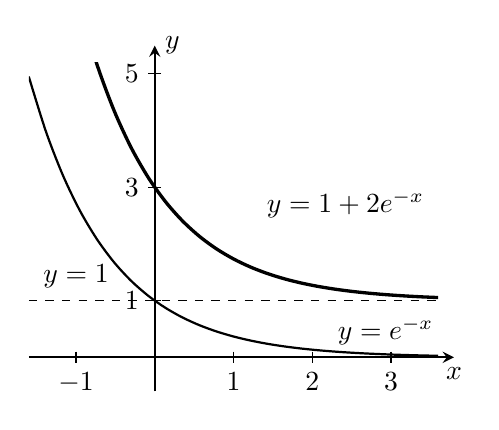
\begin{tikzpicture}[x=1.0cm,y=0.72cm,>=stealth]
  \draw[thick,->] (-1.6,0) -- (3.8,0) node[below] {$x$};
  \draw[thick,->] (0,-0.6) -- (0,5.5) node[right] {$y$};
  \foreach \x in {-1,1,2,3} \draw (\x,0.1) -- (\x,-0.1) node[below] {$\x$};
  \foreach \y in {1,3,5} \draw (0.08,\y) -- (-0.08,\y) node[left] {$\y$};
  \begin{scope}
    \clip (-1.6,-0.5) rectangle (3.6,5.2);
    \draw[thick,domain=-1.6:3.6,smooth,variable=\x] plot ({\x},{exp(-\x)});
    \draw[very thick,domain=-1.6:3.6,smooth,variable=\x] plot ({\x},{1+2*exp(-\x)});
  \end{scope}
  \draw[dashed] (-1.6,1) -- (3.6,1);
  \node[above] at (-1.0,1.05) {$y=1$};
  \node[right] at (1.3,2.7) {$y=1+2e^{-x}$};
  \node[above right] at (2.2,0.05) {$y=e^{-x}$};
\end{tikzpicture}
\end{center}
\end{solbox}

\begin{example}
দেখাও যে $y = \ln (2x)$ লেখচিত্রটি $y = \ln x$-এর একটি অনুভূমিক সংকোচন, আবার
একই সঙ্গে একটি উল্লম্ব স্থানান্তরও।
\end{example}

\begin{solbox}
$\ln(2x)$ হলো $\ln$-এর ভেতরে $x$-এর জায়গায় $2x$ বসানো, তাই সংজ্ঞা অনুযায়ী এটি
অনুভূমিকভাবে দ্বিগুণ সংকোচন।

অন্যদিকে লগারিদমের যোগের নিয়ম বলছে
\[
  \ln (2x) = \ln 2 + \ln x ,
\]
অর্থাৎ একই লেখচিত্র $y = \ln x$-কে $\ln 2 \approx 0.693$ একক উপরে সরালেও পাওয়া
যায়। দুটি বর্ণনাই সঠিক এবং একই বক্ররেখা দেয়।

এটি লগারিদমের একটি বিশেষ ধর্ম, সব ফাংশনের নয়। এর ফলে লগারিদমীয় লেখচিত্র দেখে
বলা যায় না যে $x$ কোন এককে মাপা হয়েছে; একক বদলালে গোটা বক্ররেখা কেবল উপরে বা
নিচে সরে যায়, আকার বদলায় না।
\end{solbox}

\prob{2} $y = \ln x$ থেকে $y = 2 - \ln (x+1)$ পেতে কী কী রূপান্তর, কোন ক্রমে
প্রয়োগ করতে হবে? নতুন ফাংশনের domain ও vertical asymptote বলো, এবং সে বর্ধমান
না হ্রাসমান তা বলো।

\begin{sol}
ক্রম: প্রথমে $\ln(x+1)$, অর্থাৎ ১ একক বামে সরানো; তারপর $-\ln(x+1)$, অর্থাৎ
$x$-অক্ষে প্রতিফলন; শেষে $2 - \ln(x+1)$, অর্থাৎ ২ একক উপরে সরানো।

Domain: $\ln$-এর ভেতরের রাশি ধনাত্মক হতে হবে, তাই $x + 1 > 0$, অর্থাৎ
$x > -1$। Vertical asymptote $x = 0$ থেকে সরে $x = -1$ হয়েছে। যেহেতু $\ln x$
বর্ধমান এবং প্রতিফলন চিহ্ন উল্টে দেয়, নতুন ফাংশনটি হ্রাসমান।
\end{sol}

\prob{2} $y = e^{x}$ লেখচিত্রকে পরপর (ক) $y$-অক্ষে প্রতিফলন, (খ) ৩ একক ডানে
স্থানান্তর, (গ) ১ একক নিচে স্থানান্তর করা হলো। ফলে পাওয়া বক্ররেখার সমীকরণ,
range এবং horizontal asymptote নির্ণয় করো।

\begin{sol}
(ক)-এর পরে $y = e^{-x}$। (খ)-এর পরে $x$-এর জায়গায় $x - 3$ বসে, তাই
$y = e^{-(x-3)} = e^{3-x}$। (গ)-এর পরে
\[
  y = e^{3-x} - 1 .
\]
$e^{3-x}$ সবসময় ধনাত্মক, তাই range হলো $(-1, \infty)$, এবং horizontal
asymptote $y = -1$।
\end{sol}

\prob{3} $c$ একটি ধ্রুবক।
\begin{enumerate}
  \item দেখাও যে $y = e^{x+c}$ লেখচিত্রটি $y = e^{x}$-এর একটি অনুভূমিক
        স্থানান্তর, আবার একই সঙ্গে একটি উল্লম্ব প্রসারণও; প্রসারণের গুণক কত?
  \item $f$ এমন একটি ফাংশন হলে, যার জন্য প্রতিটি অনুভূমিক স্থানান্তর কোনো না
        কোনো উল্লম্ব প্রসারণের সমান, তবে $f$-এর কী ধর্ম থাকতে হবে? উপরের
        উদাহরণ থেকে অনুমান করো।
\end{enumerate}

\begin{sol}
\begin{enumerate}
  \item $e^{x+c}$ মানে $x$-এর জায়গায় $x + c$ বসানো, অর্থাৎ $c$ একক বামে
        স্থানান্তর ($c > 0$ হলে)। আবার সূচকের নিয়ম থেকে
        $e^{x+c} = e^{c} \cdot e^{x}$, অর্থাৎ একই বক্ররেখা $y = e^{x}$-কে
        উল্লম্বভাবে $e^{c}$ গুণ প্রসারিত করলেও পাওয়া যায়। প্রসারণের গুণক
        $e^{c}$।
  \item শর্তটি হলো $f(x + c) = M(c) \, f(x)$ আকারের একটি সম্পর্ক, যেখানে
        গুণক $M(c)$ কেবল $c$-এর উপর নির্ভর করে, $x$-এর উপর নয়। এটিই এই
        অধ্যায়ের প্রথম অনুচ্ছেদে দেখা সূচকীয় ফাংশনের চরিত্র। অর্থাৎ
        ধর্মটি সূচকীয় ফাংশনেরই বৈশিষ্ট্য।
\end{enumerate}
তুলনা করে দেখো: $\ln$-এর ক্ষেত্রে অনুভূমিক \emph{প্রসারণ} উল্লম্ব
\emph{স্থানান্তরের} সমান হয়েছিল, কারণ $\ln$ গুণকে যোগে নামায়। দুটি ফলই একই
সম্পর্কের দুই পিঠ।
\end{sol}

\section{জোড় ও বিজোড় ফাংশন}

\begin{idea}[জোড় ও বিজোড়]
ধরি $f$-এর domain প্রতিসম, অর্থাৎ $x$ domain-এ থাকলে $-x$-ও থাকে। তাহলে
\begin{enumerate}
  \item $f$ কে বলা হয় জোড় (even) যদি সব $x$-এর জন্য $f(-x) = f(x)$;
  \item $f$ কে বলা হয় বিজোড় (odd) যদি সব $x$-এর জন্য $f(-x) = -f(x)$।
\end{enumerate}
জোড় ফাংশনের লেখচিত্র $y$-অক্ষ সাপেক্ষে প্রতিসম; বিজোড় ফাংশনের লেখচিত্র মূলবিন্দু
সাপেক্ষে প্রতিসম, অর্থাৎ $180^{\circ}$ ঘোরালে সে নিজের উপরেই পড়ে।
\end{idea}

\begin{center}
\begin{tikzpicture}[>=stealth]
 \begin{scope}[x=0.8cm,y=0.40cm]
  \draw[thick,->] (-2.7,0) -- (2.9,0) node[below] {$x$};
  \draw[thick,->] (0,-1) -- (0,7.4) node[right] {$y$};
  \draw[thick,domain=-2.5:2.5,smooth,variable=\x] plot ({\x},{\x*\x});
  \draw[dashed] (-1.6,0) -- (-1.6,2.56); \draw[dashed] (1.6,0) -- (1.6,2.56);
  \draw[fill] (-1.6,2.56) circle (1.6pt); \draw[fill] (1.6,2.56) circle (1.6pt);
  \node at (0,-8.6) {জোড়: $f(-x) = f(x)$};
 \end{scope}
 \begin{scope}[xshift=5.6cm,x=0.8cm,y=0.40cm]
  \draw[thick,->] (-2.7,0) -- (2.9,0) node[below] {$x$};
  \draw[thick,->] (0,-7.4) -- (0,7.4) node[right] {$y$};
  \draw[thick,domain=-1.9:1.9,smooth,variable=\x] plot ({\x},{\x*\x*\x});
  \draw[dashed] (-1.6,0) -- (-1.6,-4.1); \draw[dashed] (1.6,0) -- (1.6,4.1);
  \draw[fill] (-1.6,-4.1) circle (1.6pt); \draw[fill] (1.6,4.1) circle (1.6pt);
  \node at (0,-8.6) {বিজোড়: $f(-x) = -f(x)$};
 \end{scope}
\end{tikzpicture}
\end{center}

নাম দুটি এসেছে $x^{n}$ থেকে: $n$ জোড় হলে $(-x)^{n} = x^{n}$, আর $n$ বিজোড় হলে
$(-x)^{n} = -x^{n}$। কিন্তু বেশিরভাগ ফাংশনই এই দুই দলের কোনোটিতেই পড়ে না;
যেমন $e^{x}$, কারণ $e^{-x}$ না $e^{x}$-এর সমান, না তার ঋণাত্মক।

কয়েকটি সহজ ফল, যেগুলো বারবার লাগে। বিজোড় ফাংশনের domain-এ $0$ থাকলে
$f(0) = 0$, কারণ $f(0) = f(-0) = -f(0)$ থেকে $2f(0) = 0$। গুণফলের ক্ষেত্রে
জোড় $\times$ জোড় $=$ জোড়, বিজোড় $\times$ বিজোড় $=$ জোড়, আর
জোড় $\times$ বিজোড় $=$ বিজোড়; পূর্ণসংখ্যার জোড়-বিজোড় যোগের নিয়মের মতোই মনে
রাখা যায়। প্রমাণও এক লাইনের: $f, g$ বিজোড় হলে
$(fg)(-x) = f(-x)g(-x) = (-f(x))(-g(x)) = (fg)(x)$।

\begin{example}
নিচের ফাংশনগুলো জোড়, বিজোড়, নাকি কোনোটিই নয়?
\[
  f(x) = \frac{x}{1+x^{2}}, \qquad
  g(x) = e^{x} + e^{-x}, \qquad
  h(x) = x + \cos x .
\]
\end{example}

\begin{solbox}
$f(-x) = \dfrac{-x}{1+(-x)^{2}} = \dfrac{-x}{1+x^{2}} = -f(x)$, সুতরাং $f$
বিজোড়।

$g(-x) = e^{-x} + e^{x} = g(x)$, সুতরাং $g$ জোড়। খেয়াল করো, $e^{x}$ নিজে জোড়ও
নয় বিজোড়ও নয়, অথচ এই যোগফলটি জোড়।

$h(-x) = -x + \cos(-x) = -x + \cos x$ (৭ নম্বর অধ্যায় থেকে $\cos$ জোড়)।
এটি $h(x) = x + \cos x$-এর সমান নয়, আবার $-h(x) = -x - \cos x$-এরও সমান নয়।
একটি মান দিয়ে দেখানোই যথেষ্ট: $h(1) \approx 1.54$, $h(-1) \approx -0.46$,
আর $-h(1) \approx -1.54$। সুতরাং $h$ কোনোটিই নয়।
\end{solbox}

\begin{idea}[প্রতিসাম্য কাজ কমায়]
$f$ জোড় বা বিজোড় হলে $x \geq 0$ অংশের লেখচিত্র আঁকলেই যথেষ্ট; বাকি অর্ধেক
প্রতিফলন করে পাওয়া যায়। তথ্যের দিক থেকে বললে, প্রতিসাম্য মানে অর্ধেক তথ্যই
পুরোটা ঠিক করে দেয়।
\end{idea}

এই কথাটা পদার্থবিজ্ঞানে আরও শক্তিশালী রূপে ফিরে আসে। একটি প্রতিসম আধান বিন্যাসের
ক্ষেত্রে অর্ধেক হিসাব করলেই চলে; আর ১৭ নম্বর অধ্যায়ে দেখা যাবে যে বিজোড়
ফাংশনের ক্ষেত্রে $-a$ থেকে $a$ পর্যন্ত integral সবসময় শূন্য, কারণ দুই পাশের
অবদান কাটাকাটি যায়। প্রতিসাম্য দেখে আগেই বলে দেওয়া যে একটি রাশি শূন্য, এটি
অলিম্পিয়াডে সময় বাঁচানোর সবচেয়ে বড় কৌশলগুলোর একটি।

\begin{example}
প্রতিসাম্য ব্যবহার করে $y = e^{-x^{2}}$ লেখচিত্রের আকার বর্ণনা করো।
\end{example}

\begin{solbox}
প্রথমে প্রতিসাম্য: $(-x)^{2} = x^{2}$, তাই $e^{-(-x)^{2}} = e^{-x^{2}}$, অর্থাৎ
ফাংশনটি জোড়। সুতরাং $x \geq 0$ অংশটুকু বুঝলেই হলো।

$x \geq 0$-এ $x^{2}$ বাড়ে, তাই $-x^{2}$ কমে, তাই $e^{-x^{2}}$ কমে (কারণ
$e^{u}$ বর্ধমান)। $x = 0$-এ মান $e^{0} = 1$, যা সর্বোচ্চ। $x$ বড় হলে $-x^{2}$
অনেক নিচে নামে, তাই মান দ্রুত $0$-এর দিকে যায়, কিন্তু কখনো $0$ হয় না।

সুতরাং লেখচিত্রটি $y$-অক্ষ সাপেক্ষে প্রতিসম, $(0,1)$ বিন্দুতে সর্বোচ্চ, দুই
দিকেই দ্রুত নেমে $x$-অক্ষের দিকে যায়। এটিই ঘণ্টা আকৃতির সেই বক্ররেখা, যা
পরিসংখ্যান ও তাপগতিবিদ্যায় বারবার আসে।
\end{solbox}

\prob{2} প্রতিটি ফাংশন জোড়, বিজোড়, নাকি কোনোটিই নয়, তা নির্ণয় করো এবং সংক্ষেপে
যুক্তি দাও।
\begin{enumerate}
  \item $x^{4} - 3x^{2} + 1$
  \item $x^{3} + x$
  \item $x \, |x|$
  \item $\ln x$
  \item $x^{2} e^{-x^{2}}$
\end{enumerate}

\begin{sol}
\begin{enumerate}
  \item জোড়: প্রতিটি ঘাত জোড় (ধ্রুবককে $x^{0}$ ধরা যায়), তাই $x$-এর জায়গায়
        $-x$ বসালে কিছুই বদলায় না।
  \item বিজোড়: $(-x)^{3} + (-x) = -(x^{3}+x)$।
  \item বিজোড়: $(-x)|-x| = -x|x|$, কারণ $|-x| = |x|$।
  \item কোনোটিই নয়, এবং কারণটা সংজ্ঞাগত: $\ln$-এর domain $(0,\infty)$ প্রতিসম
        নয়, তাই প্রশ্নটাই অর্থহীন হয়ে যায়। $f(-x)$ লেখাই সম্ভব নয়।
  \item জোড়: $x^{2}$ জোড় এবং $e^{-x^{2}}$ জোড়, আর জোড় $\times$ জোড় $=$ জোড়।
\end{enumerate}
\end{sol}

\prob{3} ধরি $f$-এর domain প্রতিসম।
\begin{enumerate}
  \item দেখাও যে $f$-কে সবসময় একটি জোড় ও একটি বিজোড় ফাংশনের যোগফল হিসেবে লেখা
        যায়, এবং এই ভাঙা একমাত্র উপায়ে হয়।
  \item $f(x) = e^{x}$-এর ক্ষেত্রে এই দুটি অংশ বের করো। এদের নাম যথাক্রমে
        $\cosh x$ ও $\sinh x$ (hyperbolic cosine ও hyperbolic sine)।
  \item প্রমাণ করো যে $\cosh^{2} x - \sinh^{2} x = 1$।
\end{enumerate}

\begin{sol}
\begin{enumerate}
  \item \textbf{অস্তিত্ব।} ধরি
        \[
          E(x) = \frac{f(x) + f(-x)}{2}, \qquad
          O(x) = \frac{f(x) - f(-x)}{2} .
        \]
        তাহলে $E(-x) = \dfrac{f(-x)+f(x)}{2} = E(x)$, অর্থাৎ $E$ জোড়; এবং
        $O(-x) = \dfrac{f(-x)-f(x)}{2} = -O(x)$, অর্থাৎ $O$ বিজোড়। যোগ করলে
        $E(x) + O(x) = f(x)$।

        \textbf{একমাত্রতা।} ধরি $f = E + O$ যেখানে $E$ জোড় ও $O$ বিজোড়। তাহলে
        $f(-x) = E(x) - O(x)$। এই দুটি সমীকরণ যোগ ও বিয়োগ করলে
        $E(x) = \dfrac{f(x)+f(-x)}{2}$ এবং $O(x) = \dfrac{f(x)-f(-x)}{2}$,
        অর্থাৎ উপরের রাশি দুটিই একমাত্র সম্ভাবনা।
  \item $f(x) = e^{x}$ হলে $f(-x) = e^{-x}$, তাই
        \[
          \cosh x = \frac{e^{x} + e^{-x}}{2}, \qquad
          \sinh x = \frac{e^{x} - e^{-x}}{2},
        \]
        এবং $e^{x} = \cosh x + \sinh x$।
  \item সরাসরি হিসাব:
        \[
          \cosh^{2} x - \sinh^{2} x
          = \frac{\left( e^{x}+e^{-x} \right)^{2} - \left( e^{x}-e^{-x} \right)^{2}}{4}
          = \frac{4 \, e^{x} e^{-x}}{4} = e^{0} = 1 .
        \]
        মাঝের ধাপে ৩ নম্বর অধ্যায়ের $(p+q)^{2} - (p-q)^{2} = 4pq$ অভেদটি
        ব্যবহার করা হয়েছে।
\end{enumerate}
\end{sol}

\begin{remark}
শেষ সমস্যাটি ছোট হলেও তাৎপর্যপূর্ণ। $\cosh^{2} - \sinh^{2} = 1$ দেখতে
$\cos^{2} + \sin^{2} = 1$-এর মতো, কেবল একটি চিহ্ন আলাদা; এই মিলটা কাকতালীয় নয়,
আর ১৮ নম্বর অধ্যায়ে জটিল সংখ্যা হাতে এলে দেখা যাবে যে দুটি আসলে একই
সম্পর্কের দুই চেহারা। ততক্ষণ পর্যন্ত এটুকু মনে রাখলেই যথেষ্ট যে $e^{x}$-কে
জোড় ও বিজোড় অংশে ভাঙলে দুটি নতুন এবং কাজের ফাংশন পাওয়া যায়।
\end{remark}

\end{document}